\section{Edge Detection}
Edge detection, as the name implies, attempts to detect edges in an image. This can be done in many different ways, some of which are introduced in \cref{ssc:edge_preprocessing}, \nameref{ssc:edge_preprocessing}. However, to use edge detection for recognition, the detected edges needs to be described in some way for recognition algorithms to understand the data. Methods to perform this description are presented in section \cref{ssc:edge_based_segmentation}.

\subsection{Preprocessing}\label{ssc:edge_preprocessing}
Preprocessing covers the detection of edges and is needed before edges in an image can be described and analysed. The preprocessing detects edges to determine certain properties. This is done with operators, some of which are described in the following. Furthermore, other aspects have influence on detecting edges. These aspects are mentioned after the introduction of the operators.

\subsubsection{Operators}
Preprocessing includes a number of operators which calculates gradient for a given pixel. Gradient defines how an image is changing in regards to colour or illumination. The gradient is defined by two aspects, gradient magnitude and gradient direction. Magnitude is the rate at which the change is happening, and direction tells in which direction the illumination or colour levels rises. The direction has offset in the horizontal axis, meaning a direction to the right is 0\degree. The degrees then follow the rotational direction which is counter clockwise, as an example 180\degree is directly left.
 
In order to gather the gradient information, it is not enough to look at each pixel alone, therefore most operators work with a 3x3 mask, which is a region of 9 pixels. The center pixel is the pixel of interest and the surrounding pixels are used for references.

Since pixels are to be analysed, there must exist a way to identity each pixel. Images are often split up like coordinate systems, where each pixel has a unique coordinate, annotated $(x,y)$. X is the horizontal position and y is the vertical position. The offset for the enumeration is in the upper left corner, so the upper left pixel is denoted $p=(0,0)$, whereas the bottom right pixel is denoted $p=(x_{max}, y_{max}) $.

The operators are designed to compare pairs of pixels around the chosen pixel. The operators either look in a \textit{4-neighbourhood} or \textit{8-neighbourhood}. For a 4-neighbourhood it means the operators solely look horizontally and vertically, using the pixels left and right of the center pixel, and directly above and below the center pixel. The 8-neighbourhood looks in the same directions as the 4-neighbourhood, and in addition to this it looks on the diagonal pixels.

\textbf{An example}

The following example serves to illustrate the use of mask and gradient.
Consider an image that is ½ white and ½ black, with the white half at the top of the image. In most gray-scale images, white is fully bright and black is of no brightness\citep{gray_scale_brightness}. This means white has a value of 255 and black has a value of 0. If looking at a black pixel on the border between the black and white, the gradient direction is 90\degree\ as the gradient levels increases in a north direction, which corresponds to 90\degree. The 3x3 mask is placed with the pixel in the center. The gradient magnitude can then be calculated by the formula $mag(x,y)=\sqrt{dy^2+dx^2}$. $dx$ is calculated by subtracting the pixel to the right of the center-pixel with the pixel the the left of the center pixel, and $dy$ is calculated by subtracting the pixel above with the pixel below. 

Calculating $dx$ and $dy$ will in the example yield $dx=0-0$ and $dy=255-0$, so there is no change in the horizontal(x) direction, which follows the border. There is, however, a big change in the vertical(y) direction, which makes sense because the pixel is on the border between white and black.

\textbf{Laplacian operator}

The laplacian operator calculates the magnitude of pixels. It can be used when the gradient magnitude is the only value of interest, as it does not take any regards for direction. It is often used with the aforementioned 3x3 mask and can be used to look either in a 4- or 8-neighbourhood. One disadvantage is that it looks twice at some edges.
The Laplacian operator is often used for image sharpening, which is intended to sharpen edges to be more visual for the human eye.

\textbf{Compass operators}

A specific subset of operators is called compass operators as they estimate the gradient direction together with the magnitude. All the operators work with a 3x3 mask, and some allow larger masks to be used. Most operators calculate gradient magnitude for all pairs of opposite pixels in the border of the mask and the greatest magnitude then defines the gradient direction.
In addition, some compass operators define the direction by three pixels in each direction, where the gradient magnitude for the negative direction(towards darker areas) are negated, as illustrated in \cref{fig:mask_dir}.
Some operators differ in the way that they utilise all eight pixels in the mask border to define the gradient direction, where three pixels are used for negative direction(illustrated with -1) and five for the positive direction. Another difference is an operator which also marks direction by three pairs of pixels but the operator only detects horizontality or verticality of edges. This means that the resulting image for horizontality only has horizontal lines, and vertical lines are drawn using short horizontal edges, over the span of the vertical line, and horizontal lines will appear as is, and vice versa for verticality.
\begin{figure}[H]
	\centering
	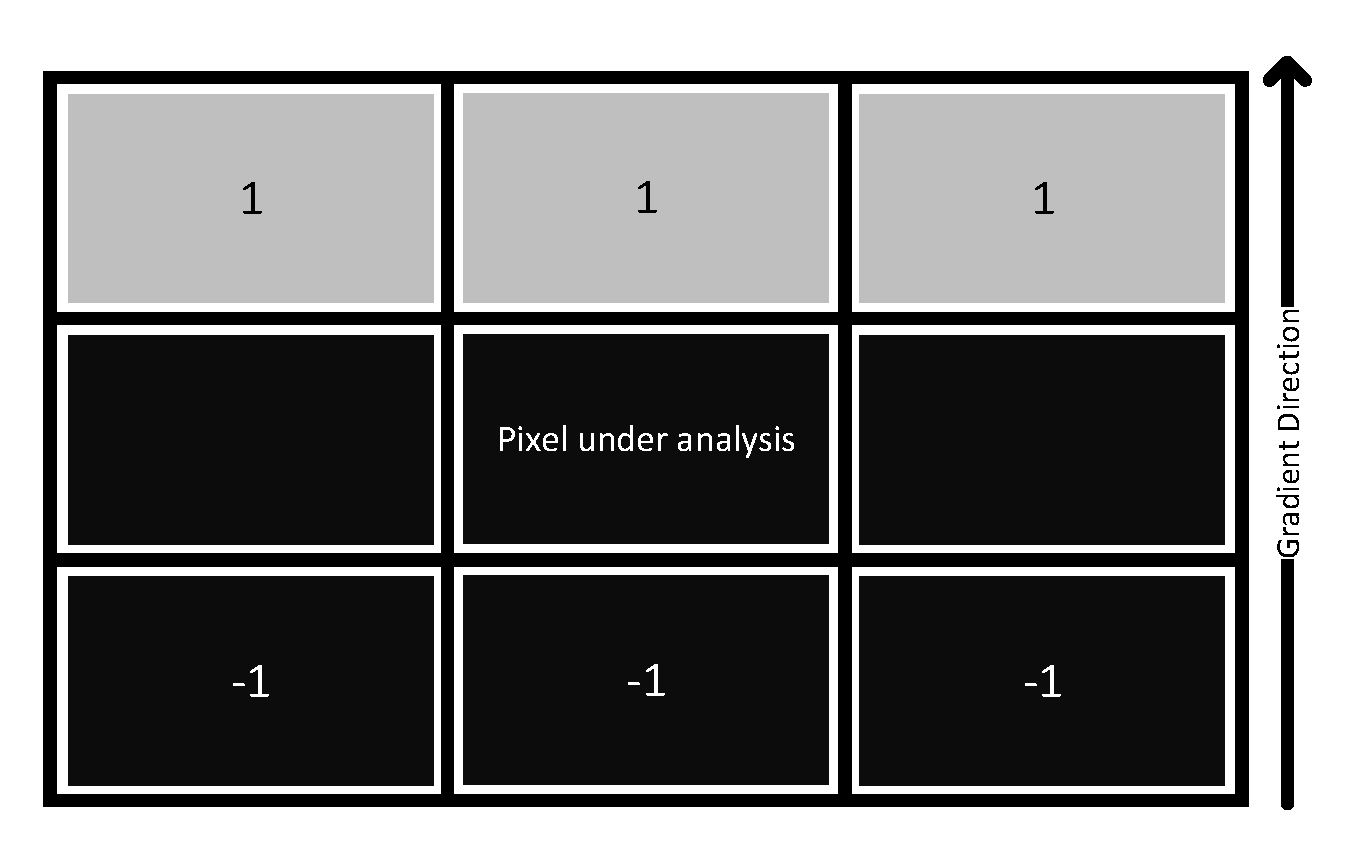
\includegraphics[width=0.5\textwidth]{graphics/mask_directed.pdf}
	\caption{Weighted values corresponding to gradient direction}
	\label{fig:mask_dir}
\end{figure}

\subsubsection{Scale}
Most image analysis methods, including edge detection, works locally. Increasing the scale gives a larger locality, as the analysed neighbourhood is increased, which in turn can give more precise estimates. However, the neighbourhood can also become too large and detail is lost, as some edges can be ignored either because of noise from other segments or because the details themselves are seen as noise.
If a large scale or possibly a global scale is to be used, the same problems of implementing \gls{ai} as mentioned in \cref{ssc:loc_glo_view} will occur. The optimal scale when working locally varies across the analysis of an image, as some parts might need more details to be captured, and some parts like a thick edge would need more scale to be recognised correctly.

\subsubsection{Edge profiles}
Edge detection can be improved by applying an edge profile, which defines the type of edges that is searched for. Two such profiles are illustrated in \cref{fig:roof_profile} and \ref{fig:step_profile}. The roof profile \cref{fig:roof_profile} is often used when detecting thin lines, whereas the step profile \cref{fig:step_profile} can be used in situations where there is a great difference in a region and the surrounding region.
\begin{figure}[H]
    \begin{minipage}{0.5\textwidth}
    	\centering
    	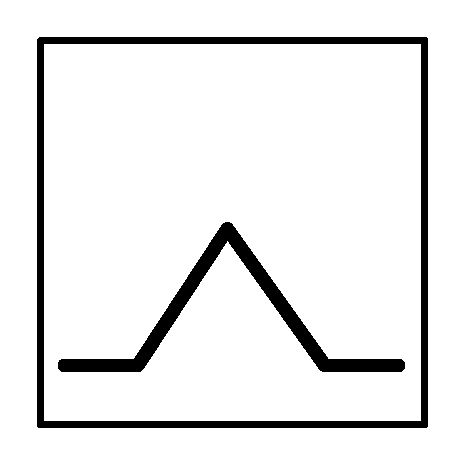
\includegraphics[width=0.80\textwidth]{graphics/roof_profile.pdf}
    	\caption{Roof profile}
    	\label{fig:roof_profile}
    \end{minipage}%
	\begin{minipage}{0.5\textwidth}
    	\centering
    	
\includegraphics[width=0.80\textwidth]{graphics/step_profile.pdf}
    	\caption{Step profile}
    	\label{fig:step_profile}
	\end{minipage}
\end{figure}


\subsubsection{Multi-spectral images}\label{ssc:m-s_images}
The edge detection described so far covers images in a single spectral range, such as grayscale images. Multi-spectral images includes RGB images and light frequencies out of the human visual range, such as infra-red. When working with multi-spectral images the different spectral bands must be analysed, for RGB, meaning the red, the green, and the blue spectral bands. This can be done in various ways, one of which is to analyse edges in each individual spectrum and combine the partial results for a final result. Other methods include using the difference of gradients between two spectres or using a multi-spectral edge detector which uses gradient information from all spectral bands.

\subsubsection{Edge Detection Using Threshold}\label{ssc:edge_threshold}
Threshold is an old technique for segmenting objects and background mainly in grayscale images. It is inexpensive and fast to execute but works best if objects are separated and there is a distinct difference in the brightness levels of the objects and their background. Choosing a proper threshold value is a necessity for a correct segmentation, as a low threshold will lose segmentations and a high threshold will include too much information.
Furthermore, a single threshold is rarely enough for an image. Often there are both lower- and upper-bound values, but the optimal segmentation value can also vary across an image. As mentioned, threshold segmentation is mainly used for gray-scale images, but can also be used in multi-spectral images in the same ways as explained in \cref{ssc:m-s_images} for multi-spectral images.

\subsection{Edge-based segmentation} \label{ssc:edge_based_segmentation}
The edge detection methods described hitherto detect edges and cannot solely be used for describing edges and borders in an image. So far each individual pixel has been analysed to see whether this pixel can be part of the edge of an object. The next step is to connect the edge pixels, while also keeping in mind some of these might be noise. Describing edges covers ways to specify how edges are to be interpreted in an image. Two separated circles on a uni-coloured background must be described as separate circles. Different edges on the border of each circle must be connected such that the circle can be described as a whole. This results in two circular segments with the background being a third segment. There are different ways to perform such a segmentation. The rest of this section explains how the segmentation can be done based on the edges that has been detected.

To do this segmentation, other methods can be applied for combining detected edges into edge chains that corresponds better with actual lines in the image. An edge chain contains information to describe how edges are connected to each other. One way to do this notation is to use numbers 0-7 to specify a direction, where 0 is right, 1 is upper right, 2 is up, and so on.
Using an edge pixel as reference, the chaining can then begin by noting what position the starting pixel is in, and noting what direction the next edge pixel is. If the chain at some point arrives at the reference pixel again, a complete segment has been found. This chaining can then be done for all edges.

Another method for edge-based segmentation is \textit{edge relaxation}, which analyses a central edge that is an edge in the crack between two pixels, illustrated with features on \cref{fig:crack_edge}. The central edge is connected to three cracks on each side and with knowledge from these six cracks, edge relaxation is able to determine if the central crack edge is part of an edge border.
The belief of the crack edge being a border edge is denoted by a confidence level, which depends on the information gathered from neighbouring cracks. For example, if neither of the neighbouring cracks are believed to be border edges, then the belief of the central crack edge to be a border edge is zero. If some of the neighbouring cracks have edges, then the confidence that the central crack edge is a border edge is raised. To extend this method, two other crack edges parallel to the central crack edge can be added as competitors to which the central edge must have a greater confidence level.

\begin{figure}[H]
	\centering
	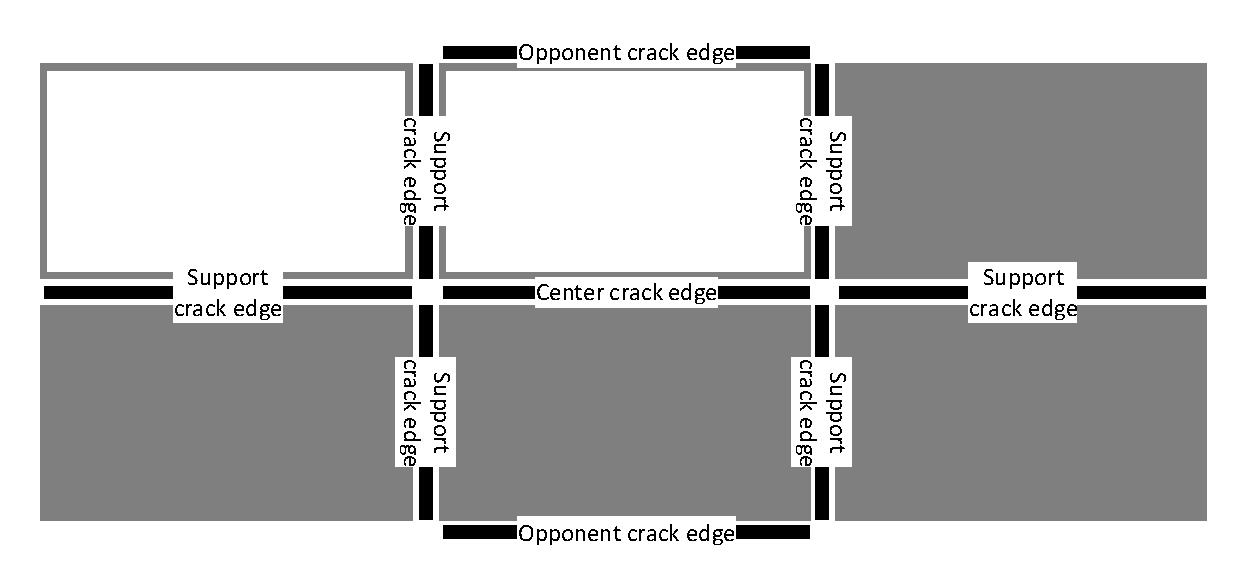
\includegraphics[width=0.5\textwidth]{graphics/crack_edges.pdf}
	\caption{Illustration of crack edge and supportive features}
	\label{fig:crack_edge}
\end{figure}

The methods described so far detects borders which partially or completely segments the given image. If this segmentation is complete, the edges outline all the regions in the image. However, if some borders are partial, the determination of regions is  complex, as it often requires higher-level information about the object, such as shape and size. Even with this information, the partial regions might not be acceptable; several regions can be blurred together and seen as one. A method of determining regions from the partial segments is to compare segments from different threshold values. Another method which includes the gradient direction considers a closest opposite edge pixel, by searching in a straight line which may have a maximum distance \textit{M} between them following the negative gradient direction of border pixel, a simple illustration is shown in \cref{fig:partial_region}. If two edge pixels can be connected this way, those two and all pixels in the line between them are marked as region members. If a pixel gets atleast three marks, it is considered a region member, otherwise it is marked as a background pixel. The \textit{M} distance is often chosen from knowledge of the size of the regions of the object that is of interest.

\begin{figure}[H]
	\centering
	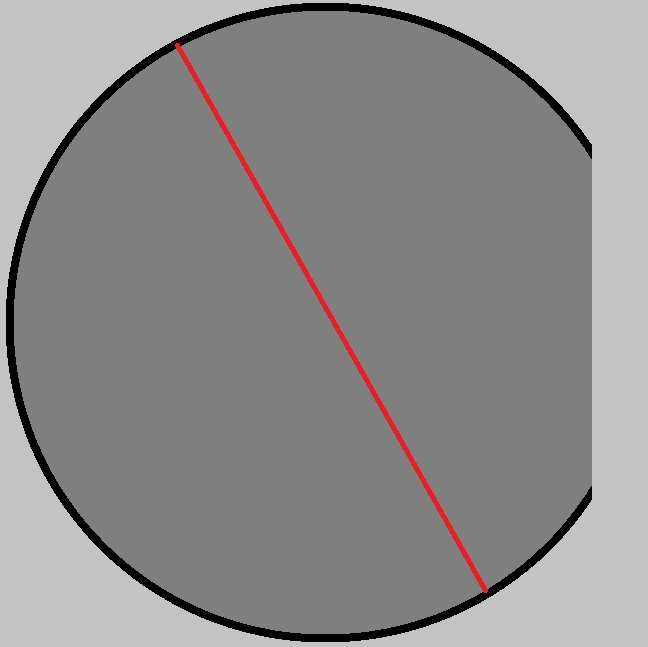
\includegraphics[width=0.5\textwidth]{graphics/partial_region.jpg}
	\caption{Simple illustration of opposite pixel pair in partial region}
	\label{fig:partial_region}
\end{figure}